\documentclass[a4paper,11pt]{article}
\usepackage[utf8]{inputenc}
\usepackage[T1]{fontenc}
\usepackage[french]{babel}
\usepackage[right=2.5cm, left=2.5cm, bottom=4cm, top=3cm]{geometry}
\usepackage[ddmmyyyy]{datetime}
\usepackage[table]{xcolor}
\usepackage{lmodern,mathptmx,changepage,titlesec,hyperref,listings,lstautogobble,graphicx,array,longtable,multirow,lipsum,tikz,shorttoc,enumitem,float}
\usetikzlibrary{arrows,automata}
\usetikzlibrary{positioning}

\renewcommand{\rmdefault}{\sfdefault} %Utilisation de la police sans-serif ("Computer Modern Sans") pour la police roman
\renewcommand{\ttdefault}{pcr} 	%Utilisation d'une police "CourrierNew" pour la police monospaced (pour faire un listing manuel)
\linespread{1.15}				%Interligne

%Utilisation de liens colorés en bleu et soulignés
\hypersetup{colorlinks=true, urlcolor=blue, urlbordercolor=blue, linkcolor=black, linkbordercolor=white}
\makeatletter \Hy@AtBeginDocument{\def\@pdfborder{0 0 1} \def\@pdfborderstyle{/S/U/W 1}}\makeatother

\titlespacing*{\section} {0cm}{7ex plus 1ex minus .2ex}{1.5ex plus .2ex}
\titlespacing*{\subsection} {0cm}{4.5ex plus 1ex minus .2ex}{1.5ex plus .2ex}
\titleformat*{\section}{\LARGE\bfseries}
\titleformat*{\subsection}{\large\bfseries}
\titleformat*{\subsubsection}{\normalsize\bfseries}

\definecolor{darkgreen}{rgb}{0,0.8,0}
\definecolor{mygray}{rgb}{0.93,0.93,0.93}
\definecolor{mymauve}{rgb}{0.58,0,0.82}
\lstset{	
	language=Python,
	basicstyle=\small\ttfamily,
	backgroundcolor=\color{mygray},
	breaklines=true,
	breakatwhitespace=true,
	tabsize=3,
	frame=none,
	rulecolor=\color{black},
	keywordstyle=\color{blue}\bfseries,
	stringstyle=\color{orange},
	showstringspaces=false,
	commentstyle=\footnotesize\color{darkgreen},
	keepspaces=true,
	extendedchars=true,
	numbers=left,
	numberstyle=\tiny\color{lightgray},
	stepnumber=1,
	escapeinside={(@}{@)},
	autogobble=true,
	literate=
		{á}{{\'a}}1 {é}{{\'e}}1 {í}{{}}1 {ó}{{\'o}}1 {ú}{{\'u}}1
		{Á}{{\'A}}1 {É}{{\'E}}1 {Í}{{\'I}}1 {Ó}{{\'O}}1 {Ú}{{\'U}}1
		{à}{{\`a}}1 {è}{{\`e}}1 {ì}{{\`i}}1 {ò}{{\`o}}1 {ù}{{\`u}}1
		{À}{{\`A}}1 {È}{{\'E}}1 {Ì}{{\`I}}1 {Ò}{{\`O}}1 {Ù}{{\`U}}1
		{ä}{{\"a}}1 {ë}{{\"e}}1 {ï}{{\"i}}1 {ö}{{\"o}}1 {ü}{{\"u}}1
		{Ä}{{\"A}}1 {Ë}{{\"E}}1 {Ï}{{\"I}}1 {Ö}{{\"O}}1 {Ü}{{\"U}}1
		{â}{{\^a}}1 {ê}{{\^e}}1 {î}{{\^i}}1 {ô}{{\^o}}1 {û}{{\^u}}1
		{Â}{{\^A}}1 {Ê}{{\^E}}1 {Î}{{\^I}}1 {Ô}{{\^O}}1 {Û}{{\^U}}1
		{œ}{{\oe}}1 {Œ}{{\OE}}1 {æ}{{\ae}}1 {Æ}{{\AE}}1 {ß}{{\ss}}1
		{ç}{{\c c}}1 {Ç}{{\c C}}1 {ø}{{\o}}1 {å}{{\r a}}1 {Å}{{\r A}}1
		{€}{{e}}1 {£}{{\pounds}}1 {«}{{\guillemotleft}}1
		{»}{{\guillemotright}}1 {ñ}{{\~n}}1 {Ñ}{{\~N}}1 {¿}{{?`}}1
}

%Redéfinition de la taille de \Huge pour le titre du document
\makeatletter\renewcommand\Huge{\@setfontsize\Huge{37pt}{40}}\makeatother
\date{\today}


\title{\vspace{\fill}\textbf{\Huge Rapport Semestre 2}}
\author{Jean-Didier Pailleux - Maxence Joulin - Damien Thenot - Romain Robert - Robin Feron 
	\vspace{2em}\\
	\textit{Test de primalité}\\
	\textcolor{red}{https://github.com/CHPS-M1-PRIME-NUMBERS/Prime\_numbers}
	\vspace{2em}
}
\usepackage{algorithm}
\usepackage{algorithmic}
\usepackage{subcaption}
\begin{document}
\pagenumbering{gobble}\clearpage
\maketitle\vspace{13em}
\begin{center}
\includegraphics[scale=0.7]{logo.png}\end{center}
\begin{flushright}\textit{Projet de Programmation numérique}\end{flushright}
\newpage
\tableofcontents
\newpage\clearpage\pagenumbering{arabic}

	\section{Introduction}
	\paragraph{}Ce document est le compte rendu de notre travail qui s'inscrit dans le cadre de la deuxième période du module \textit{Projet de Programmation numérique} du master \textit{Calcul Haute Performance Simulation} de l'\textit{\textbf{UVSQ}} proposé par notre encadrant Sébastien Gougeaud.
	
	\paragraph{}Durant la première période de ce projet, il nous a été demandé d'implémenter plusieurs tests de primalité en séquentiel dans le but de déterminer si un grand nombre donné est premier ou non. On rappelle qu'un nombre premier est un entier qui admet uniquement deux diviseurs distincts et positifs: 1 et lui-même. Il existe deux types de tests de primalité, les déterministes qui permettent d'établir avec certitude le résultat et les tests probabilistes qui émettent un résultat non fiable avec une certaine probabilité d'erreur, mais possèdent de meilleures performances que les tests déterministes.

	\paragraph{}Ce projet est une application de plusieurs algorithmes (AKS, Miller-Rabin, Pocklington, Euclide et Ératosthène) pour tester la primalité d'un nombre. Après une étude des tests effectués durant la première période sur un échantillon de valeurs, nous avons pu faire plusieurs comparaisons entre ces méthodes et l'on a pu observer que les méthodes naïves sont très utiles pour les petits nombres, mais deviennent très lentes pour de très grands nombres. De plus, Miller-Rabin est un test probabiliste intéressant du fait qu'il ait une exécution très rapide avec une probabilité très faible d'obtenir un résultat erroné. Cependant, notre implémentation de l'algorithme de AKS ne fût pas très performante dû à l'utilisation de la bibliothèque NTL pour l'arithmétique modulaire.
	
	\paragraph{}L'objectif de cette deuxième période consiste en premier lieu à optimiser si possible les algorithmes utilisés puis de s’occuper de faire tourner plusieurs de ces tests en parallèle et ainsi évaluer la scalabilité de nos implémentations. Le parallélisme de calculs et de données seront utilisés. Pour le parallélisme de données le problème de l'équilibre de charge se posera. De plus, pour effectuer nos tests, plusieurs visites à la Maison de la Simulation seront faites pour y faire tourner sur un supercalculateur cette nouvelle version de notre programme. 
	
	\paragraph{}Dans la première partie de ce document, on présentera les différentes optimisations appliquées sur les tests de notre projet.
	Après cela, on mentionnera les différents outils et le modèle utilisé au cours de la phase de l'implémentation de la parallélisation dans une partie Parallélisation. Puis dans une autre partie l'analyse des résultats établis lors des tests du projet accompagné d'un comparatif avec sa version séquentielle.
	Finalement, dans les deux dernières parties, on établira un bilan quant à l'organisation interne au sein du groupe pour cette deuxième période et un bilan technique suite à l'observation des résultats qui mettra en avant les limites des outils utilisés.
	
		
	\section{Optimisation}
	Pour débuter cette deuxième période il nous fallait d'abord commencer l'optimisation des différents tests de primalité implémentés. Le premier test étant le \textit{eratosthene()} dont le premier problème concerne la mémoire utilisée. En effet, un nombre premier ne peut être un nombre pair hormis $2$. Pour un très grand nombre $N$ donné, $\frac{N}{2}-1$ nombres entre 1 et N sont pairs et non-premier ce qui correspond à un espace mémoire de $4*(\frac{N}{2}-1)$ octets utilisés inutilement dans le tableau de booléen de la fonction \textit{eratosthene()} pour indiquer si un nombre est premier. Pour résoudre cela nous avons donc divisé par deux la taille du tableau utilisé pour ne plus prendre en compte les nombres paires. Cette observation économise 50\% de mémoire et est presque deux fois plus rapide que l'algorithme de base tout en ne nécessitant que des modifications mineures du code.\\
La seconde optimisation de cette fonction concerne la boucle interne. En effet, dans la version basique, il nous arrive de visiter plusieurs fois la même case du tableau de booléen. Pour cela nous ne faisons plus $N$ itération mais $\sqrt{N}-3$ itérations.

	\paragraph{} AKS, étant un algorithme qui prenait beaucoup de temps à s'exécuter, nous avons décidé de l'optimiser. Pour cela nous avons d'abord effectué un profilage du code avec \textit{gprof} pour observer quelles sont les fonctions qui prennent le plus de temps dans l'exécution. C'est sans surprise que la partie cinq de l'algorithme (la seule partie qui utilise NTL) occupe quasiment la totalité du temps d'exécution. Le tableau ci-dessous montre un aperçu du profil d'AKS: \\
\\
\renewcommand{\arraystretch}{1.5} %donne la distance entre les lignes%
\setlength{\tabcolsep}{0.3cm} %donne la distance entre les collones%
{\footnotesize\begin{tabular}[b]{|>{\centering}m{1.5cm}|>{\centering}m{1.5cm}|>{\centering}m{1.5cm}|>{\centering}m{1.0cm}|>{\centering}m{1.5cm}|>{\centering}m{1.0cm}|>{\centering\arraybackslash}m{3.5cm}|}
\hline
\textbf{\% time} & \textbf{cumulative secondes} & \textbf{self seconds} & \textbf{calls} & \textbf{total ms/Call} & \textbf{ms/call} & \textbf{name}\\
 \hline
100.15 & 0.01 & 0.01 & 213844 & 0.00 & 0.00 & NTL::operator== \\
\hline 
0.00 & 0.01 & 0.00 & 427689 & 0.00 & 0.00 & NTL::WrappedPtr \\
\hline 
0.00 & 0.01 & 0.00 & 213844 & 0.00 & 0.00 & NTL::operator!=\\
\hline 
0.00 & 0.01 & 0.00 & 74203 & 0.00 & 0.00 &  unsigned long modpow()\\
\hline
\end{tabular}
}
\\
\\
Nous avons donc choisi d'implémenter une variante d'AKS en sélectionnant celle qui serait la plus faible en terme de complexité et qui utiliserait le moins possible la bibliothèque NTL. Pour rappel, NTL est une bibliothèque haute performance qui nous permet d'implémenter facilement des calculs modulaires sur les polynômes. Une variante sortait du lot : la Conjecture d'Agrawals\cite{Conjecture1}\cite{Conjecture2}. C'est un algorithme très performant avec une complexité en $O (log$ $n)^3$. Cependant, ce dernier est non prouvé, car à partir d'un certain rang, il existerait une infinité de contres exemples. Un projet appelé \textit{distributed computing project Primaboinca} a pour but de trouver les contres exemples de cette conjecture et affirme uniquement leur inexistence pour $n < 10^{12}$. Or, notre projet étant limité à $2^{64}$, nous pouvons donc utiliser cet algorithme sans risque d'avoir des résultats faussés.  
\begin{algorithm}
\caption{AKS Conjecture}

\begin{algorithmic}
\STATE a. Vérifier si n n'est pas un Perfect power
\STATE b. r = 2
\STATE c. Trouver r, tel que r ne divise pas $n^2 - 1$
\STATE d. Vérifier que  $(x - 1)^n \equiv x^n - 1\pmod {x^r - 1,n} $
\end{algorithmic}
\end{algorithm}

Après optimisation, on obtient un algorithme efficace qui nous permet de tester de grands nombres dans un temps raisonnable. Avec cette optimisation, on passe d'une complexité de $O (log n)^{12}$ (AKS 2002) à $O (log n)^3$. Voici l'algorithme :

	\paragraph{}Ensuite, nous avons l'algorithme de Pocklington qui repose sur la factorisation en nombres premiers, qui même avec un algorithme optimisé tel que le crible quadratique, se trouve être un problème appartenant à la classe NP. C'est-à-dire qu'il appartient aux problèmes les plus difficiles en informatique, car ceux-ci augmentent très rapidement en temps d'exécution en fonction de l'entrée de façon exponentielle. De plus, l'implémentation des algorithmes de factorisation en nombres premier plus efficace représente un problème, car ils sont basés sur des principes mathématiques difficiles à implémenter. Enfin, l'algorithme de Miller-Rabin ne peut être davantage optimisé.
	

	\section{Parallélisation}
	Après avoir optimisé notre code, nous nous sommes consacrés à la parallélisation de celui-ci. Deux types de parallélismes nous ont été proposés par notre encadrant. Le premier étant le parallélisme de calculs dans le cas où le(s) test(s) implémenté(s) nous le permettait et le parallélisme de données pour distribuer les données contenues dans une plage au sein des processus disponibles lors du lancement du programme et à y opérer les mêmes opérations (les tests de primalité ici).

		\subsection{Outils utilisés}
Pour produire cette nouvelle version du projet, certains outils ont été utilisés pour obtenir le résultat présenté. En premier lieu, nous avons utilisé \textbf{OpenMP}\cite{omp}, un API employé pour le calcul parallèle sur des architectures à mémoire partagée. Nous l'utilisons pour le parallélisme de calculs pour les fonctions de memory\_bound() et eratosthene(). L'avantage de ce dernier nous permet de rajouter des "\#pragma" sans pour autant modifier le code séquentiel.

		\paragraph{}Le deuxième outil \textbf{MPI}(Message Passing Interface)\cite{MPI} est une norme définie par une bibliothèque de fonctions utilisées pour le passage de messages entre processus. Le choix d'utiliser MPI provient du fait que cette norme est adaptée pour des machines massivement parallèles à mémoire distribuée, ce qui est le cas du supercalculateur situé à la Maison de la Simulation. Cela nous a donc permis d'exploiter au maximum les ressources mises à disposition lors de l'utilisation de cette machine. 
		
		\subsection{Parallélisme de calculs}		
	Pour le parallélisme de calculs plusieurs algorithmes tels qu'AKS et la conjecture ne supportent pas ce type de parallélisme. Pour le test de Miller-Rabin, nous avons parallélisé les k itérations permettant d'affiner la précision de l'algorithme. Après cette parallélisation nous avons effectué des tests de performance. Ces tests montraient que cette modification n'améliorait pas le temps d'exécution de l'algorithme, mais qu'au contraire elle l'augmentait. Pour cette implémentation, nous avions remplacé les valeurs de retours qui étaient des booléens par des entier 0 pour vrai et 1 pour false, ainsi les différents cœurs se répartissant les itérations faisaient la somme des valeurs de retours et lorsque cette somme était supérieure à 0 le nombre testé n'était donc pas premier. L'idée était donc ensuite d'utiliser la version optimale de Miller-Rabin avec le système master/slave pour avoir de meilleurs temps.
	
	\paragraph{}Une parallélisation possible de Pocklington semblait intéressante. Dans un premier temps, nous avons utilisé OpenMP pour la parallélisation des tests sur les facteurs premiers $N-1$. Cette tentative ne donna cependant aucun résultat intéressant. En effet, cela nous a donc fait perdre la possibilité d'arrêter l'exécution lorsque l'une des vérifications était fausse. Une majeure partie du temps de calcul se trouvant dans la factorisation en nombre premier de $N-1$, la parallélisation des tests sur les facteurs premiers et la perte de la fin sur une règle non respectée ne donne pas de résultats intéressants. 
	
	\paragraph{}Enfin, le crible d’Ératosthène (Memory Bound) est donc le seul test dont nous avons implémenté un parallélisme de calculs. Pour paralléliser cette fonction nous avons utilisé OpenMp. Pour cela, nous avons placé un \textit{\#pragma omp parallel for} pour paralléliser l'initialisation du tableau de booléen, puis
\textit{\#pragma omp parallel for schedule(dynamic)}	pour la partie appliquant l'algorithme du crible. L'utilisation de "schedule(dynamic)" indique qu'OpenMP affecte une itération à chaque thread. Lorsque le thread finit, il lui sera affecté l’itération suivante qui n’a pas encore été exécutée. Cela permet donc d'avoir une bonne répartition des tâches sur l'ensemble des threads, car on suppose que le temps de traitement pour une itération n'est pas constant.
	
		\subsection{Parallélisme de données}
		La majorité de nos tests n'étant pas parallélisés, il fallait donc opter pour un autre type de parallélisme qui est celui de données. Pour cela nous sommes donc partis sur un modèle basé sur le Master Slave (Maître-Esclave), c'est-à-dire qu'un processus sera désigné en tant que Maître et sera chargé de distribuer du travail aux esclaves qui vont donc demander à l'inverse du travail au Maître dès qu'il est libre. Le choix de ce modèle vient du fait qu'il est principalement utilisé pour une application décomposable en différentes tâches indépendantes (chaque test de primalité étant indépendant). De plus, il est nécessaire de faire attention à l'équilibre de charges, car lorsque nous donnons une plage de données à analyser, il nous est impossible de prévoir à l'avance le temps mis pour le traitement d'un nombre et donc de répartir de façon équitable le travail sur les processus. 
Pour notre implémentation, le processus Maître correspond au rang 0, il ne lancera jamais de tests de primalité (avec 4 processus, seulement 3 lanceront des tests de primalité). Le rang Maître envoie seulement un paquet d'un seul entier. Des tentatives d'envoyer des paquets de 10, 100 ou plus n'ont pas influencé le temps d'exécution final du programme. Cela peut se justifier par le fait que le temps de communication d'un message MPI était négligeable par rapport au reste (de l'ordre de $10^{-4}$s).

	\section{Analyse des résultats}
	Pour cette deuxième période du projet, l'accès au cluster \textbf{Poincare}\cite{poincare} disponible à la Maison de la Simulation du CEA nous a permis de faire plusieurs vagues de tests de scalabilité sur la version parallèle de notre projet.
	
		\subsection{Lancement d'un test}
Pour commencer ces tests nous devions charger les modules indispensables à l'utilisation de notre programme dans l’environnement utilisé avec  \textit{module load tool}. Les modules utilisés lors des tests sont \textit{gnu-env/5.4.0} et \textit{openmpi/1.10.0\_gnu54}. Lancer un test sur Poincare nécessite d'utiliser un script nommé \textit{batch.sh}, celui-ci indique donc pour un job lancé, le nombre de processus MPI (total\_tasks), le nombre de nœuds nécessaire (node, 16 tâches MPI pour 1 nœud), la durée maximum avant que le job soit tué (wall\_clock\_limit), le type de job (job\_type = mpich si parallel ou serial sinon),etc. Pour soumettre un tel job la commande \textit{llsubmit batch.sh} est utilisé. Cependant les sorties standard n'existant pas sur le cluster, des fichier job\_name.err et job\_name.log servent donc à les remplacer. Voici un exemple de fichier batch.sh :\\
	 \begin{figure}[!ht]	
		\begin{center}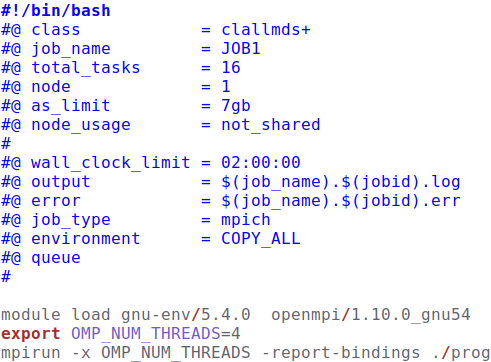
\includegraphics[scale=0.6]{batch.png}\end{center}
		\caption{Exemple de fichier batch.sh}
		\label{fg:bat}
\end{figure}
		\subsection{Résultats}
	
Tout d'abord, nous avons réalisé une première batterie de tests sur une première plage de nombres allant de 1 à 1 million avec 10 itérations. Les \textbf{Figures \ref{fg:fig1}, \ref{fig:2} et \ref{fig:3}} représentent donc l'évolution du temps de calcul en fonction du nombre processus sur cette plage. Cependant, deux tests de primalité n'ont pas eu de résultats dus à un manque de temps et aussi à leur problème de performance. Pour la première plage avec $4h$ donné lors de la soumission du job Pocklington et AKS n'ont pas pu finir leur exécution avant d'être tué par le supercalculateur quel que soit le nombre de processus donné. 
		
\begin{figure}[!ht]	
		\begin{center}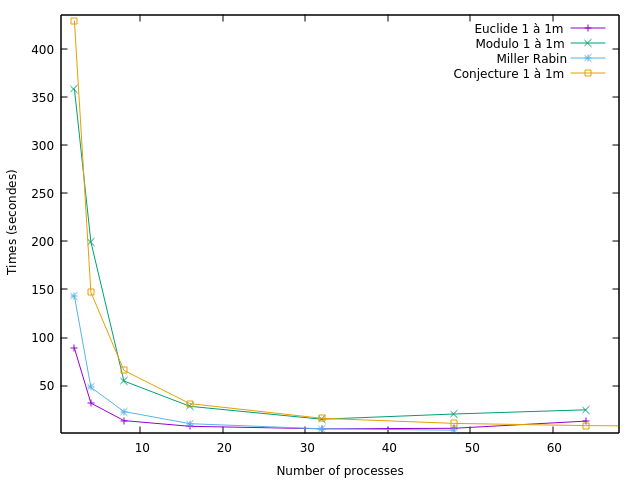
\includegraphics[scale=0.8]{All_1M.png}\end{center}
		\caption{Évolution du temps de calcul pour Conjecture, Miller-Rabin, Euclide et Modulo. }
		\label{fg:fig1}
\end{figure}

\begin{figure*}
        \centering
        \begin{subfigure}[b]{0.85\textwidth}
            \centering
            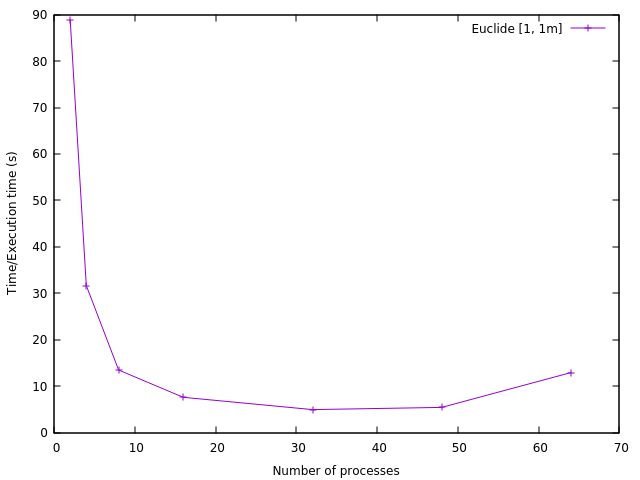
\includegraphics[width=\textwidth]{Euclide_1M.png}
            \caption[Network2]%
            {{\small Euclide}}    
            \label{fig:sub1}
        \end{subfigure}
        \hfill
        \begin{subfigure}[b]{0.85\textwidth}  
            \centering 
            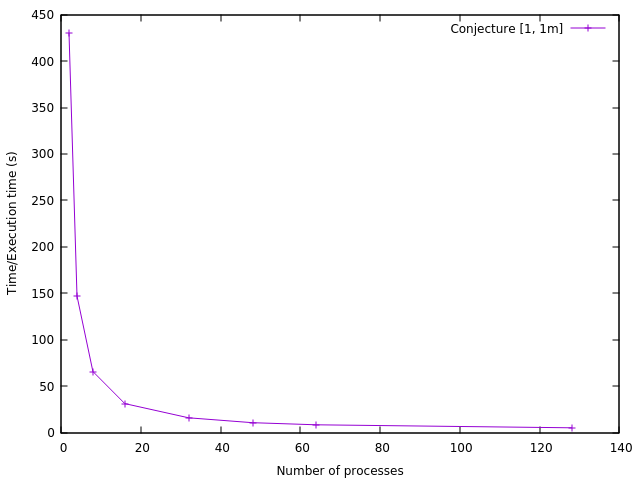
\includegraphics[width=\textwidth]{Conjecture_1M.png}
            \caption[]%
            {{\small AKS Conjecture}}    
            \label{fig:sub2}
        \end{subfigure}
         \caption[ Évolution du temps de calcul en fonction du nombre processus]
        {\small Évolution du temps de calcul en fonction du nombre processus : Plage [1, 1 000 000]} 
        \label{fig:2}
\end{figure*}
\begin{figure*}
        \begin{subfigure}[b]{0.85\textwidth}   
            \centering 
            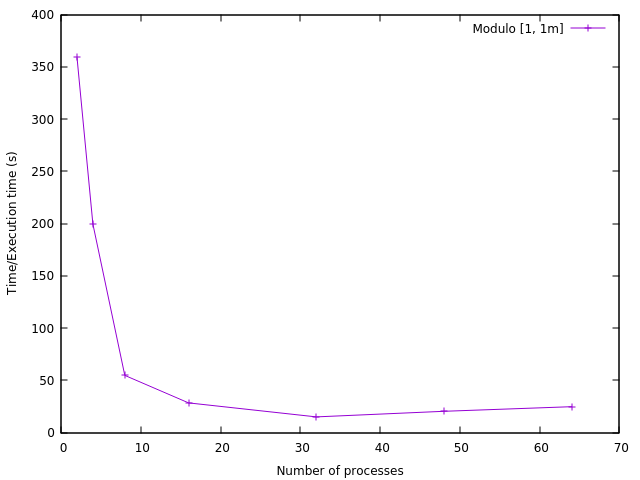
\includegraphics[width=\textwidth]{Modulo_1M.png}
            \caption[]%
            {{\small Modulo}}    
            \label{fig:sub3}
        \end{subfigure}
        \hfill
        \begin{subfigure}[b]{0.85\textwidth}   
            \centering 
            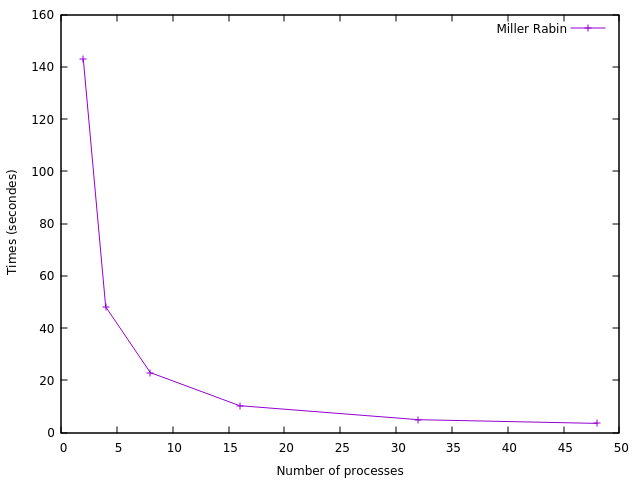
\includegraphics[width=\textwidth]{Miller.png}
            \caption[]%
            {{\small Miller-Rabin}}    
            \label{fig:sub4}
        \end{subfigure}
        \caption[ Évolution du temps de calcul en fonction du nombre processus]
        {\small Évolution du temps de calcul en fonction du nombre processus : Plage [1, 1 000 000]} 
        \label{fig:3}
\end{figure*}

D'après ces résultats nous pouvons voir que l'implémentation du modèle Master-Slave montre une bonne scalabilité. De plus, la \textbf{Figure \ref{fg:fig1}} indique que lorsque nous augmentons le nombre de processus les tests les plus lents tel que la Conjecture ont un temps d'exécution équivalent aux tests les plus rapide. Nous avons donc comparé les résultats obtenus avec ceux de notre code séquentiel (\textbf{cf. Figure \ref{fg:bar}}). La Conjecture lui va donc tourner avec $424.5s$ en moyenne, Miller-Rabin avec $129.1s$, Euclide avec $89.9s$ et Modulo avec $375s$. Cette comparaison montre qu'à partir de 3 processus MPI utilisés le programme s'exécute plus rapidement sur cette plage de données.
\begin{figure}[!ht]	
		\begin{center}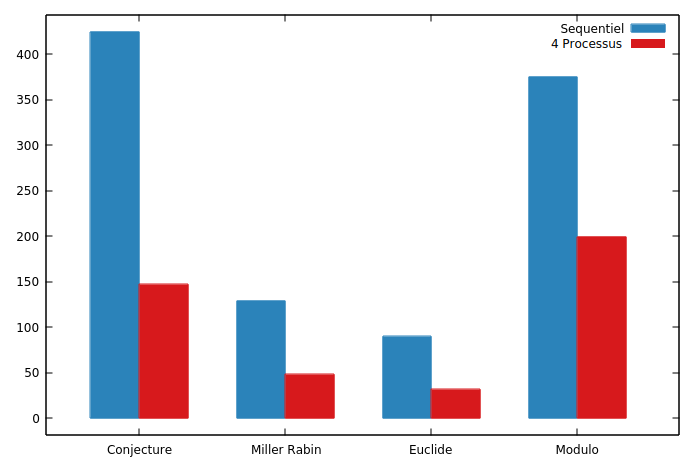
\includegraphics[scale=0.6]{Bar1.png}\end{center}
		\caption{Comparaison Conjecture, Miller-Rabin, Euclide et Modulo. }
		\label{fg:bar}
\end{figure}

Cependant, en ce qui concerne la plage [1, 1 000 000] nous pouvons observer qu'au bout d'un certain nombre de processus, il devient peu avantageux d'augmenter ce nombre. La cause de cette augmentation serait les communications MPI qui prennent le dessus sur le temps d'exécution final. En effet, les nombres de cette plage sont très petits, l'exécution d'un test serait donc beaucoup trop rapide.\\


% PLAGE 4M à 4M1m
	\paragraph{}Ensuite, nous avons réalisé une deuxième vague de tests sur une deuxième plage de nombres allant de 4 Milliard à 4 Milliard 1 million (4M1m) avec 10 itérations. Les \textbf{Figures \ref{fig:4} et \ref{fig:5}} représentent donc l'évolution du temps de calcul en fonction du nombre processus sur cette plage. Par manque de temps, le test de Miller-Rabin n'a pas pu avoir de résultat pour cette plage de données.

\begin{figure*}
        \centering
        \begin{subfigure}[b]{0.85\textwidth}
            \centering
            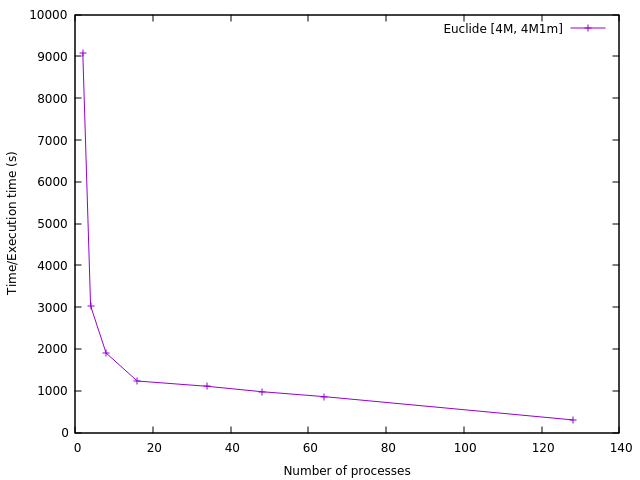
\includegraphics[width=\textwidth]{Euclide_4M.png}
            \caption[Network2]%
            {{\small Euclide}}    
            \label{fig:sub4}
        \end{subfigure}
        \hfill
        \begin{subfigure}[b]{0.85\textwidth}  
            \centering 
            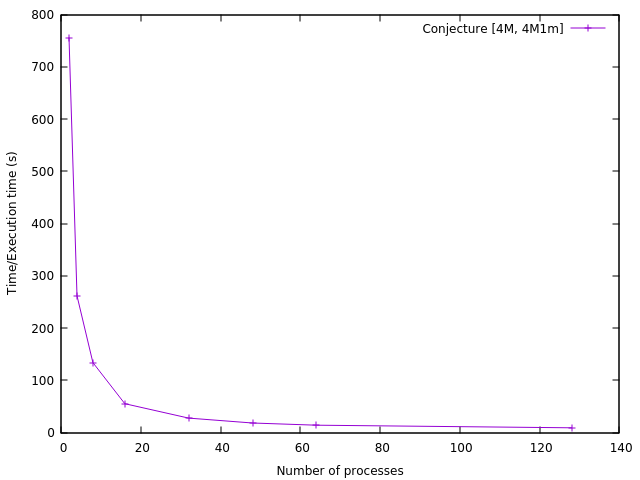
\includegraphics[width=\textwidth]{Conjecture_4M.png}
            \caption[]%
            {{\small AKS Conjecture}}    
            \label{fig:sub5}
        \end{subfigure}
         \caption[ Évolution du temps de calcul en fonction du nombre processus]
        {\small Évolution du temps de calcul en fonction du nombre processus : Plage [4M, 4M1m]} 
        \label{fig:4}
\end{figure*}
\begin{figure*}
            \centering 
            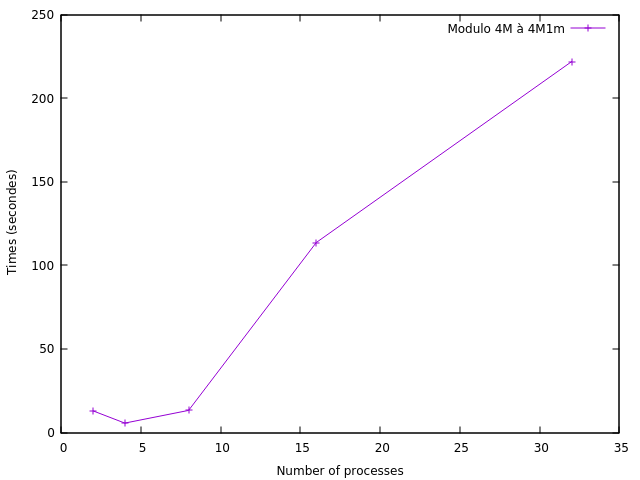
\includegraphics[width=0.8\textwidth]{Modulo_4M.png}
        \caption[ Évolution du temps de calcul en fonction du nombre processus]
        {\small Évolution du temps de calcul en fonction du nombre processus Modulo: Plage [4M, 4M1m]} 
        \label{fig:5}
\end{figure*}
	
\begin{figure*}
        \centering 
            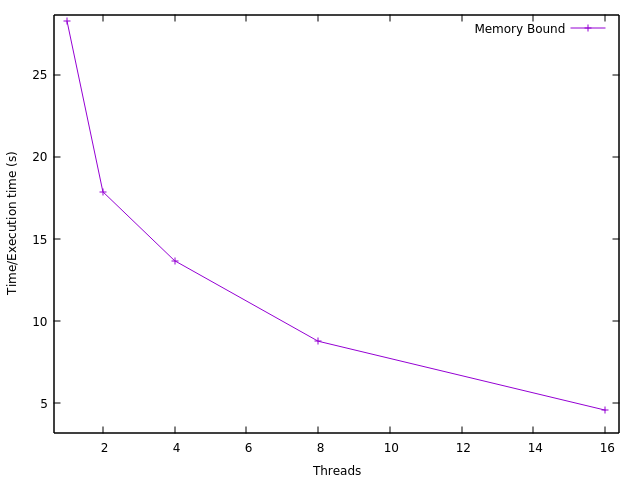
\includegraphics[width=0.8\textwidth]{Memory.png}
        \caption[Évolution du temps de calcul en fonction du nombre processus]
        {\small Évolution du temps de calcul en fonction du nombre processus pour Memory Bound : Plage [1, 500 000 000]} 
        \label{fig:6}
\end{figure*}

	Pour cette plage de données, nous pouvons voir que l'implémentation possède toujours une bonne scalabilité à l'exception du résultat pour Modulo. D'après notre encadrant Matthieu Haefele ce résultat serait causé par l'utilisation de nœuds qui ne serait pas saines lors de nos tests. Ce résultat ne serait pas causé par notre implémentation et donc ne sont pas représentatif.\\
	
	Les tests concernant MemoryBound (\textbf{Figure \ref{fig:6}}) ont été faits à part des autres étant donné que ce test utilise un autre type de parallélisme et qu'il calcule les nombres premier compris entre 1 et N. Les résultats de la parallélisation associés à ce test nous indique qu'il supporte plutôt bien le parallélisme de calculs même si la scalabilité affichée de celui-ci n'est pas parfaite. De plus, l'optimisation faite nous permet donc d'économiser de la mémoire au niveau de la RAM.
	\section{Bilan Technique}	
		
Suite à nos résultats, nous pouvons conclure que notre implémentation d'une communication Maitre-Esclave pour paralléliser nos recherches de nombres premiers est relativement efficaces.
L'augmentation du nombre de cœurs de calcul diminue bien par la même échelle le temps nécessaire à la recherche des nombres premiers d'une plage donnée.
On remarque cependant que cette augmentation de l'efficacité atteint un palier pour la plupart de nos tests. Selon notre analyse des temps passés dans les différentes parties de notre programme, il semblerait que le processus Maître, qui envoie les données à traiter aux processus Esclaves, soit le responsable de ce plafonnement.
\paragraph{}En effet, avec l'augmentation du nombre de cœurs de calculs, le nombre de communications que doit effectuer le processus Maître en un instant T augmente considérablement afin d'assurer le fait qu'aucun processus n'attende trop longtemps un nouveau travail.
Or, le calcul d'une donnée étant relativement court, le processus Maître arrive à saturation avec l'augmentation du nombre de nœuds de calcul.
Notre schéma de communication arrive donc à ses limites dues au fait que des processus Esclaves vont certainement ne pas être utilisé 100\% du temps.

\paragraph{}Une optimisation de notre schéma de communication aurait pu être d'envoyer des centaines voir des milliers de données à traiter à chaque processus Esclave en un envoi.
Ceci aurait pu permettre de diminuer le nombre de communications nécessaires de la part du processus Maître et ainsi le rendre plus réactif à la demande de travail d'un nouveau processus Esclave.
Cette implémentation n'a été testée que sur nos ordinateurs personnels (avec seulement 8 cœurs) et n'a cependant pas donné de résultats probants en gain de performance.

\paragraph{}Une autre implémentation aurait pu être réalisée en augmentant le nombre de processus Maître. En effet, en divisant la taille du problème en plusieurs processus Maîtres, on aurait divisé d'autant la charge qui pèse sur leurs épaules.

\paragraph{}Concernant l'équilibrage des charges sur nos processeurs, il est important de rappeler que nos calculs sont très courts, de l'ordre d'un centième de seconde pour la plupart de nos algorithmes d'évaluation.
Ainsi, un cœur ne prendra pas beaucoup plus de temps qu'un autre pour analyser sa donnée, même si celle-ci demande plus de temps pour déterminer sa primalité.
Notre équilibrage de charge est donc presque parfait, de l'ordre de 1/10ème de seconde de différence entre les deux processus les plus éloignés en terme de fin d’exécution pour 40 secondes de temps total d’exécution. Donc aucun équilibrage compliqué n'a été nécessaire.

\paragraph{}Le problème de recherche des nombres premiers dans une plage de donnée est donc hautement parallélisable et notre implémentation en Maitre/Esclave est efficace. Cependant, la limite de ce problème réside avant tout dans la non-parallélisation des tests en eux-mêmes dû à leur forme très simple.
Les limites techniques de rapidité de calculs sont donc rapidement atteintes et seul l'augmentation du volume de donnée laisserait entrevoir l'utilité de l'augmentation du nombre de nœuds de calcul et leur bonne utilisation.		
		
	\section{Problèmes rencontrés}
	Lors de nos séances à la maison de la simulation, nous avons été dans l'impossibilité d'effectuer nos tests en raison d'un problème technique au niveau des nœuds de calcul qui n'étaient plus disponibles.
	A la première séance nous avons eu besoin d'implémenter un Makefile. Nous utilisions à la base cmake qui s'occupait alors de créer le Makefile pour nous, mais cmake n'était pas compatible avec les machines auxquelles nous avions accès à la Maison de la Simulation. Lors de l'implémentation de ce Makefile nous avons rencontré des problèmes d'intégration des bibliothèques NTL et GMP, ce qui nous a retardé dans les tests.
	Enfin, lors de notre dernière séance, certains de nos résultats peuvent avoir été faussé causé par des nœuds qui n'étaient pas sain (un temps d'exécution de $300s$ au lieu de $25s$ par exemple).
					
	\section{Organisation interne du groupe}
	Pour débuter la deuxième période de ce projet, il nous fallait en premier lieu établir une nouvelle répartition du travail de groupe pour que le projet puisse avancer de façon efficace et de manière rapide. Le tableau ci-dessous va ainsi indiquer pour chaque membre du groupe la où les fonctionnalités pour lesquels il a pu contribuer. \\
	
	\begin{center}\vspace{-1em}\footnotesize\begin{longtable}{|>{\centering}m{4cm}|>{\centering}m{1.5cm}|>{\centering}m{1.5cm}|>{\centering}m{1.5cm}|>{\centering}m{1.5cm}|>{\centering\arraybackslash}m{1.5cm}|}			
		\hline \multicolumn{1}{|c|}{\textbf{Tâches}} & \multicolumn{1}{c|}{\textbf{Jean-Didier}} & \multicolumn{1}{ c|}{\textbf{Maxence}} & \multicolumn{1}{ c|}{\textbf{Romain}} & \multicolumn{1}{ c|}{\textbf{Robin}} & \multicolumn{1}{c|}{\textbf{Damien}}\\
		\hline 	Master slave & x & x & ~ & ~ & ~ \\
		\hline 	Parallélisation /Optimisation Memory Bound & x & ~ & ~ & ~ & ~ \\
		\hline 	AKS Conjecture & ~ & ~ & x & ~ & ~ \\
		\hline 	Tests parallélisation Miller-Rabin & ~ & x & ~ & x & ~ \\
		\hline 	Tests parallélisation Pocklington & ~ & x & ~ & ~ & x \\
		\hline 	Makefile & ~ & ~ & x & x & x \\
		\hline 	Rapport & x & x & x & x & x \\
		\hline 	Tests & x & x & x & x & x \\
		\hline
	\end{longtable}\vspace{-2.2em}\end{center}	
	
	\section{Conclusion}
	Pour terminer, l'utilisation de techniques de parallélisation et d'optimisation nous montre les mêmes résultats que nous avons déjà pu observer, les algorithmes les plus rapides permettent d'obtenir des résultats très rapidement sur une plage de données. Et la parallélisation mise en place permet de traiter une grande plage de données rapidement sur une machine parallèle. Cependant, les performances observées dépendent très fortement des performances individuelles des algorithmes quand on se trouve à 100\% des ressources allouées utilisés ou de l'état de "santé" des nœuds utilisés.	
	
	\paragraph{}Pour cette deuxième partie nous avons malheureusement uniquement étudié des plages de données. Nous aurions pu explorer d'autres options comme la comparaison de nos algorithmes avec des implémentations déjà existantes, mais des problèmes rencontrés à la Maison de la Simulation nous ont limité dans nos tests. Malgré cela, le résultat final reste satisfaisant, la partie parallèle est efficace, l'équilibrage de charge est très bien respectée et les optimisations effectuées ont bien amélioré les temps d’exécution.
	
	\paragraph{}Le groupe s'est une nouvelle fois très bien entendu tout au long du projet, l'entraide était vraiment présente. Pour élargir ce sujet, il serait possible d’implémenter d'autres algorithmes efficace comme ECPP(Elliptic curve primality test) ou encore APR (Adleman-Pomerance-Rumely primality test) des équivalents de l'algorithme AKS avec de bien meilleurs résultats pratiques. Mais également à d'autres schémas de parallélisation (\textit{ex: avoir plusieurs processus Maître}) du programme pour comparer les performances.
	
	\paragraph{}Ce projet nous aura donc permis d'affiner et d'améliorer nos connaissances sur la parallélisation et l'optimisation d'algorithmes, il nous aura également permis de découvrir et d'utiliser du matériel spécialisé et performant tel que le cluster Poincare du CEA. 

\bibliography{references2}
\bibliographystyle{unsrt}
\end{document}
